\documentclass[a4paper]{article}

\usepackage[utf8]{inputenc}
\usepackage[T1]{fontenc}
\usepackage{textcomp}
\usepackage{listings}
\usepackage{lmodern}
\usepackage{amsfonts}
\usepackage{titling}
\usepackage{lipsum}
\usepackage[left=1in, right=1in, bottom=1in, top=1in]{geometry}
\usepackage[backend=bibtex]{biblatex}
\usepackage{mathtools}
\usepackage{amsthm}
\usepackage{tcolorbox}
\usepackage{hyperref}
\usepackage{xcolor}
\usepackage{graphicx}
\usepackage{makeidx}
\usepackage{tikz}
\usepackage{cases}
\usepackage{apacite}
\usepackage{tkz-berge}
\usepackage{lastpage}
\usepackage{fancyhdr}
\pagestyle{fancy} 
\usepackage{url}
\usepackage{tgtermes}
\usepackage{sectsty}
\usepackage{subcaption}
\usepackage{setspace}
\usepackage{float}
\usepackage{amsmath, amssymb}
\rhead{Page~\thepage~of~\pageref{LastPage}.}
\cfoot{}

% figure support
\usepackage{import}
\usepackage{xifthen}
\pdfminorversion=7
\usepackage{pdfpages}
\usepackage{transparent}
\newcommand{\incfig}[2][1]{%
    \def\svgwidth{#1\columnwidth}
    \import{./figures/}{#2.pdf_tex}
}

%mathstyling
\theoremstyle{plain}
\newtheorem{thm}{Theorem}[section]
\newtheorem{lem}[thm]{Lemma}
\newtheorem{prop}[thm]{Proposition}
\newtheorem*{cor}{Corollary}

\theoremstyle{definition}
\newtheorem{defn}{Definition}[section]
\newtheorem{conj}{Conjecture}[section]
\newtheorem{exmp}{Example}[section]
\newtheorem{axiom}{Axiom}
\theoremstyle{remark}
\newtheorem*{rem}{Remark}
\newtheorem*{note}{Note}

\pdfsuppresswarningpagegroup=1

\begin{document}
\begin{titlepage}
\begin{center}
\large
University of Warwick \\
Department of Computer Science \\
\huge
\vspace{50mm}
\rule{\linewidth}{0.5pt} \\
CS133 \\
\vspace{5mm}
\Large
Professional Skills
\rule{\linewidth}{0.5pt}
\vspace{5mm}
\begin{figure}[H]
\centering

\includegraphics[width=0.4\textwidth]{crest_black.eps}
\end{figure}
\vspace{37mm}
Cem Yilmaz\\
\today
\end{center}
\end{titlepage}
\tableofcontents
\newpage
\section{Professional Bodies}
\subsection{Three features of a profession}
Because the definition of a "profession" varies from place to place and dictionary to dictionary, we instead cover what is common between all of them: I.e., the definitions of a profession always have:
\begin{itemize}
	\item Body of people, i.e, it is a group
	\item Self-governing i.e., it has its own control over itself
	\item Entry to profession is controlled i.e., requires a degree
\end{itemize}
\subsection{Professional Bodies}
\begin{defn}
	Profession - a paid occupation, especially one that involves prolonged training and a formal qualification.
\end{defn}
\begin{defn}
	Professional body - an organisation with individual members practicing a profession or occupation in which the organisation maintains an oversight of the knowledge, skills, conduct and practice of that profession or occupation.
\end{defn}
\subsubsection{Engineering Council}
The engineering council offers professional qualifications such as:
\begin{itemize}
	\item CEng, IEng, EngTech which are limited to UK only (awarded through BCS), 
	\item EUR ING (throughout Europe using FEANI)
\end{itemize}
with BCS (British Computer Society) being a licensed institution of the Engineering Council and it offers:
\begin{itemize}
	\item CITP (UK only)
	\item ISEB (a software engineering qualification, highly regarded)
\end{itemize}
They also have a code of conduct which has four duties:
\begin{itemize}
	\item Public Interest - regard for public health, privacy, security and well-being of environment and people
	\item Professional competence and integrity - only perform work/services within professional competence and develop skills and competence on a continuing basis
	\item Duty to Relevant Authority - carry out responsibilities with care and diligence and avoid conflicts of interest
	\item Duty to the Profession - Uphold the reputation and seek to improve standards
\end{itemize}

\subsubsection{Science Council}
Similarly for science professions, there exists the Science Council and it was incorporated in 2003. It consists of $41$ member bodies, including the IMA (Institute of mathematics and its applications). The IMA is a professional institution for scientists in a computing discipline. \\
Some qualifications include:
\begin{itemize}
	\item CSci, CSciTech, RSci, RSciTech
\end{itemize}
\subsubsection{Other Councils}
The General Medical Council regulates doctors in the United Kingdom. They set standards, hold a register, quality assure education and investigate complaints. \\
Royal College of Veterinary Surgeons (RCVS) \\
Royal Institute of British Architects (RIBA)
\subsection{Reservation of title and function}
\begin{defn}
	Reservation of title - name of a profession being restricted to those who are appropriately qualified.
\end{defn}
\begin{defn}
	Reservation of function - certain activities are restricted to those who have appropriate qualifications or members of particular professional bodies.
\end{defn}
\section{UK Law}
\subsection{Fundamentals}
The UK government is governed by the parliament which consists of two houses:\\
House of commons which is an elected lower house which makes the laws  \\
House of lords which is an appointed upper house which scrutinises and revises laws.
\subsection{Devolved Government}
However things for the UK are not so simple. We consider the following definitions:
\begin{defn}
	Crown dependency - a territory that is under the sovereignty of the British Crown but does not form part of the UK. The Crown dependencies are the Channel Islands and the Isle of Man.
\end{defn}
\begin{defn}
	Devolved parliament - A devolved English parliament is a proposed institution that would give separate decision-making powers to representatives for voters in England. Current devolved parliaments include Scotland and Wales.
\end{defn}
\begin{defn}
	Devolved assembly - Similar to parliament but instead for an assembly. It gives separate decision-making powers to representatives for voters. Devolved assembly includes Northern Ireland.
\end{defn}
\subsection{Making a law}
A parliament's main job is to create laws. The process is as follows:
\begin{enumerate}
	\item A bill is passed to the parliament which proposes a new law or a change to an existing law (Bills are introduced by govt or MPs or members of house of lords)
	\item The bill is examined by house of commons and house of lords. Each house makes changes and these must be agreed by both houses before it becomes law.
	\item There are cases when a bill can be passed without the approval of lords - if the same bill is passed in two successive years or if it is about taxes or public expenditure.
\end{enumerate}
I.e.,
\begin{enumerate}
	\item First Reading
	\item Second Reading
	\item Committee Stage
	\item Report Stage
	\item Third Reading
	\item Royal Assent
\end{enumerate}
\begin{defn}
	Primary legislation - term used to describe the main laws passed by the legislative bodies of the UK e.g. Acts of the UK Parliament, Scottish Parliament, Welsh Parliament and Northern Ireland Assembly. 
\end{defn}
\begin{defn}
	Secondary legislation - (also called 'subordinate legislation') is delegated legislation made by a person or body under authority contained in primary legislation. Typically, powers to make secondary legislation may be conferred on ministers, on the Crown, or on public bodies.
\end{defn}
\subsection{EU Law}
EU laws take immediate effect when agreed. They are self executing - an example of GDPR. \\
Furthermore, EU directives must be enacted by the individual countries. Each country makes their own law when directed to do so by the EU.
\subsection{UK Legal System}
\begin{defn}
	Adversarial System - prosecution and defence compete to determine the facts
\end{defn}
\begin{defn}
	Inquisitorial - getting the truth through enquiry and investigation
\end{defn}
The UK system is adversarial.
\subsection{Criminal Law and Civil Law}
\begin{defn}
	Criminal law - there is a presumption of innocence. The prosecution must prove 'beyond reasonable doubt' test that you are guilty. The crown prosecution service decides to move the prosecution forward. The juries decide guilt or innocence whilst the judge decides the penalty.
\end{defn}
\begin{defn}
	Civil law - the case is decided on a balance of probabilities test and concerns relationships between individuals. E.g., contracts, property, family law etc.
\end{defn}
\section{Intellectual Property}
\subsection{Tangible and Intangible}
\begin{defn}
	Tangible - a thing that is perceptible by touch. E.g., car, house, gas etc.
\end{defn}
\begin{defn}
	Intangible - unable to be touched; not having physical presence. E.g., software, literature, art etc.
\end{defn}
\begin{defn}
	Intellectual property - Intellectual property (IP) refers to creations of the mind, such as inventions; literary and artistic works; designs; and symbols, names and images used in commerce. I.e., intangible things
\end{defn}
\subsection{Copyright v Patents v Trademarks}
Copyright, patents and trademarks are all things that relate to law and intellectual property. 
\subsubsection{Copyright}
Copyright is defined as the right to copy/adapt something. This could be one of the following:\\
Book, journal, article, image, song, software etc. \\
Work with copyright allows the owner to copy, change, sell, share and rent it to others. More importantly, it can be used to prevent others from doing the same and gaining unfair benefit from your work. \\
The US favours the copyright holders using the Digital Millennium Copyright Act (DMCA) which protects the copyright \\
The World Intellectual Property Organisation (WIPO) also exists that regulates the IP. \\
Lastly, the Anti-counterfeiting Trade agreement (ACTA) came out of secret negotiations in 2011/12 and it criminalises certain classes of IP infringement e.g. downloads of movies, software etc. It puts responsibility to Internet Service Provider (ISP) responsible for users' online use. It has only been ratified in Japan.
The EU directive on copyright in 2019 created a law which:
\begin{itemize}
	\item Requires websites to obtain license from publishers to link to news stories in their sites
	\item Requires platforms to obtain licenses for content e.g., music videos
\end{itemize}
In 2014 the copyright went through a change after a result of criticism from a book. It now includes that the following uses of copied materials are permitted:
\begin{itemize}
	\item Archiving and preserving
	\item Data analysis e.g. for research
	\item Research and education as long as the source is acknowledged
	\item Private use e.g., copying a few pages of a book
	\item Accessible copies for disabled persons
\end{itemize}
\subsubsection{Trade marks}
Trade marks are protected under the Trade Marks act 1994. In the UK, the intellectual property office (IPO) adjudicates on any disputes. Registration of trade marks and designs is advisable, and is checked in disputes. However, there is a great question about how much Trade Marks Act really protects. Copyrighting a domain name works by 'grandfather rights' i.e., registration of domain in good name and there is no conflict of interest you are not infringing the legislation.
\subsubsection{Patents}
Patent confers to a temporary right to exploit an invention an usually for 20 years. In EU, the patented invention must:
\begin{itemize}
	\item Be new
	\item Involve an inventive step
	\item Be capable of industrial application
	\item Not be in an excluded area
\end{itemize}
Excluded areas include:
\begin{itemize}
	\item Scientific Theories
	\item Mathematical Methods
	\item Aesthetic creations - copyright instead
	\item Presentation of information - copyright instead
	\item Algorithms and software
\end{itemize}
A patent must be registered at the IPO. Disclosure before application invalidates a patent, therefore an invention must be kept confidential prior to patenting it. In EU, software are not patentable. However, in the US, this is allowed if the following is true
\begin{itemize}
	\item Is part of a procedure that is patentable
	\item Controls a process with physical effect
	\item Processes real physical data
\end{itemize}
\subsection{Digital Rights Management}
In the past deliberate errors were introduced to things such as books to detect copying. Today, software companies try to protect their software etc. by incorporating technology to prevent it:
\begin{itemize}
	\item Product keys - each purchaser receives a different key
	\item Limited number of active installations - i.e., max 3
	\item Presistent online authentication - it continually checks that it is authorised i.e., DRM
\end{itemize}
\subsection{Whistle-Blowing}
Confidentiality fails under the following conditions (Public Interest Disclosure Act 1998):
\begin{itemize}
	\item Criminal offense
	\item Failure to comply with legal obligation
	\item Miscarriage of justice
	\item Environmental damage
	\item Health and safety
	\item Concealment of any of the above
\end{itemize}
\subsection{Registration requirement}
The following require registration:
\begin{itemize}
	\item Registered trade marks
	\item Registered designs
	\item Patents
	\item Domain names
\end{itemize}
And the following are automatically protected:
\begin{itemize}
	\item Unregistered trade marks
	\item Unregistered design rights
	\item Confidential information
	\item Copyright
\end{itemize}
\section{Data Protection}
Data theft can cause damage financially, through fraud or embarrassment.
\subsection{Problem}
Types of data that can be hacked, accidentally lost or altered. For example through:
\begin{itemize}
	\item Credit Card theft
	\item Identity theft
	\item Sensitive personal information
	\item Tracking by unauthorised agencies e.g. purchasing behaviour, travel
\end{itemize}
\subsection{TalkTalk}

Information commissioners office (ICO) issued a fine of $400,000$ GBP to TalkTalk, a company whose investigation found that an attack last October could have been prevented if TalkTalk had taken basic steps to protect customers' information. The ICO found that the cyber attack between 15 to 21 October 2015 took advantage of the companies' weak systems. The data of 156,959 people was stolen including their numbers, addresses, names, email addresses. In 15,656 cases, the attacker gained access to bank account details and sort codes. \\
\subsection{Facebook}
In September 2018, $50m$ Facebook accounts were compromised by an attacker that gave hackers the ability to take over' others' accounts. Users that were affected were notified by facebook and required to log out and log back in. They also stole access tokens - a kind of security key that allows users to log back into the app without having to enter password every time.
\subsection{Solution}
In 1984, computers stored medical and financial data and then it was realised that potential problems this could occur. As a result, the Council for Europe Convention was introduced which enables discussions between governments on matters of mutual interests. In 1998, the EU Data Protection Directive lead to the 1998 Data protection Act. The GDPR Data Protection Regulation in $2016$ forms part of the Data Protection Act. These regular how data is stored and who can access the data. 
\begin{defn}
	Personal data - data that is stored and processed about a data subject (a real person). GDPR refers to 'any information'
\end{defn}
\begin{defn}
	Data subject - An 'identified or identifiable natural person'
\end{defn}
\begin{defn}
	Information Commissioner - a person who makes sure data is correctly supervised under law
\end{defn}
\begin{defn}
	Processing - anything to do with data, e.g., storage, collection, recording or organising.
\end{defn}
\begin{defn}
	Controller - can be a person, authority or body that determines the prepose and means of the processing of personal data.
\end{defn}
1998 Data Protection Act superseded the 1984 act. The DPA 1998 refers to the accessible records and relevant filing systems e.g. filing cabinets not just computerised data. 
\subsection{Jurisdiction and Enforcement}
The GDPR (General Data Protection Regulation) applies to any organisation anywhere in the world if data is collected relating to any EU resident.The GDPR enforces penalties for violations of obligations and legal justification up to $20m$ euros or $4\%$ of global gross revenue. The GDPR enforces penalties for breaching GDPR for up to $10m$ euroes or up to $4\%$ of global gross revenue.
\subsection{Data Protection Officer}
The following organisations require data protection officer:
\begin{itemize}
	\item All entities involved with 'regular and systematic monitoring of data subjects on a large scale'
	\item All public authorities
	\item All entities conducting large-scale processing of 'special categories of personal data' e.g., racial/ethnic origin, political beliefs, religious beliefs etc.
\end{itemize}
\subsection{Data Breaches}
Data breaches must be reported within $72$ hours. Privacy impact assessments must be made (if appropriate) focusing on protecting data subjects' rights.
\begin{defn}
Pseudonymisation - the processing of personal data in such a manner that the personal data cano no longer be attributed to a specific data subject without the use of additional information, provided such additional information is kept separately and is subject to technical and organisational measures to ensure that the personal data are not attributed to an identified or identifiable natural person.
\end{defn}
\subsection{7 Data Protection Principles}
\begin{enumerate}
	\item Processing of personal data must be lawful, fair and transparent
	\item Purposes of processing of personal data must be specified, explicit and legitimate
	\item Personal data must be adequate, relevant and not excessive
	\item Personal data must be accurate and kept up to date
	\item Personal data must be kept for no longer than is necessary
	\item Personal data must be processed in a secure manner
	\item The controller is accountable
\end{enumerate}
\subsection{Lawfulness of processing}
Data can be 'lawfully' processed if:
\begin{itemize}
	\item Necessary for performance of a contract
	\item Legal obligations
	\item 'Vital interests' of a data subject
	\item Public interest or official authority
	\item Consent of data subject
	\item 'Legitimate interests'
\end{itemize}
However, note that consent to processing must be freely given, should be specific and informed, not be ambiguous and must have 'legitimate interests'
\subsection{Exemptions}
Exemptions for consentual data include:
\begin{itemize}
	\item Legal privilege
	\item Taxation
	\item Self incrimination
	\item Immigration
	\item Journalism
	\item Research
	\item Parliamentary privilege
	\item Employment references
	\item Exam scripts and marks
	\item Social work data
	\item health data
\end{itemize}
\subsection{Right of Access to Data}
You have right to access data/information about yourself as a result of GDPR:
\begin{itemize}
	\item Right of access by the data subject (normally within 1 month)
	\item Right to rectification
	\item Right to erasure (right to be forgotten)
	\item Right to restriction of processing
	\item Right to data portability
	\item Right to object to automated profiling
\end{itemize}
However, note that you do not have right to view information about yourself that the police has if you are under investigation.
\subsection{Profiling}
\begin{defn}
	Profiling - the activity of collecting information about someone
\end{defn}
Certain types of profiling is considered problematic - consider how insurance companies arrive at how much you pay based on your medical data, health, economic situation and reliability. You have a right not to subject to profiling, but it is not yet $100\%$ clear in legal terms. A good example of profiling is personalised advertising.
\subsection{Privacy}
Issue of privacy is extremely complicated and is complex. For the sake of this module we only consider Regulation of Investigatory Powers Act 2000 (RIPA). It sets up a framework for controlling the lawful interception of computer, telephone and communications. Governments can access data only in certain specified situations such as preventing and detecting crime. They are allowed to monitor and record communications without the consent.
\section{Freedom of Information}
The freedom of information act $2000$ covers all public bodies in the UK e.g., local government, NHS, universities, police, parliament etc. Furthermore it:
\begin{itemize}
	\item Extends definition of data in Data Protection Act 1998 to include 'unstructured' records
	\item Freedom of Information refers to non-personal data
	\item Freedom of Information refers to information that is not sensitive
	\item Changes 'need to know' to 'right to know'
	\item Requests are in writing (e.g. fax) or by email, stating clearly the information that you want to know
	\item Response from bodies must say if the information exists, if it does, it must be shared
	\item Bodies must give cost and time limit for request (20 working days or until fee is paid, max 3 months)
\end{itemize}
However, absolute exceptions include:
\begin{itemize}
	\item Security services
	\item Trade secrets (protecting new designs)
	\item Court records (confidential)
	\item 'Vexacious' requests (e.g., spamming a company for lots of information)
\end{itemize}
and qualified exceptions include:
\begin{itemize}
\item Subject to prejudice test (crime detection)
\item Not in the public interest
\end{itemize}
\subsection{Publication Schemes}
Freedom of Information (FOI) Act requires every public body to publish information proactively. The publication schemes should:
\begin{itemize}
\item Have list of information to be published by types of organisations
\item Need approval from Information Commissioner
\item Information that is of interest to the general public should be available
\item Use 'model publication schemes', the organisation no longer needs to respond to all requests
\end{itemize}
The Information Commissioner can adjudicate and can enforce disclosure, but the public authority's complaints process must be followed first. Lastly, the information commissioner can be overruled by an appropriate government.
\subsection{Issues}
\begin{itemize}
	\item Data sharing - the sharing of data between organisations
	\item Government disallows a request - why would it do this
	\item Credit agencies - where do credit agencies get their data
	\item DNA databases - who owns your DNA and who should be allowed to know the information
	\item Cross-border data - should different countries share information
\end{itemize}
\section{Computer Misuse}
\subsection{Computer Misuse Act (CMA) 1990}
Introduced the following case of $1987$ case of Regina vs Gold and Schifreen - stolen credentials via shoulder surfing. 
\begin{defn}
	Shoulder surfing - the practice of spying on the user of cash-dispensing machines or other electronic devices in order to obtain their personal identification number, password etc.
\end{defn}
Convictions were being overturned so new law was required to deal with the changing tech landscape. The CMA as a result was introduced with new offenses:
\begin{itemize}
	\item Unauthorised access to computer material
	\item Unauthorised access with intent to commit or facilitate further offences
	\item Unauthorised modification of computer material
\end{itemize}
\begin{defn}
	Computer System - any device or a group of interconnected or related devices, one or more of which, pursuant to a program, performs automatic processing of data.
\end{defn}
\begin{defn}
	Computer Data - any representation of facts, information or concepts in a form suitable for processing in a computer system, including a program suitable to cause a computer system to perform a function.
\end{defn}
\subsection{Offenses}

\subsubsection{Unauthorised access}
I.e., unauthorised access to computer material \\
Causing 'a computer to perform any function with intent to secure access to any program or data held in any computer' such that the access is knowingly unauthorised. The unauthorised access is the offence - not any damage done.
\subsubsection{Unauthorised access with Intent}
I.e., unauthorised access with intent to further facilitate commission of further offences. Intent to commit a crime carries a punishment of 5 year prison or more plus an unlimited fine. It is not necessary to prove that the intended further offence has actually been committed.
\subsubsection{Unauthorised modification}
I.e., unauthorised acts with intent to impair, or with recklessness as to impairing the operation of a computer. \\
The intention is to
\begin{itemize}
	\item Impair the operation of the target computer
	\item Prevent or hinder access to any program or data
	\item Impair the operation of a program or the reliability of any data
\end{itemize}
\subsubsection{Section 3ZA}
I.e., unauthorised acts causing, or creating risk of, serious damage. \\
The maximum sentence of indictment is $14$ years and an unlimited fine, unless the offense caused or created a significant risk of serious damage to human welfare or national security, in which case a person guilty of offence is liable to imprisonment for life.
\subsubsection{Note}
The location of the equipment is vague on purpose meaning that it is irrelevant where it happens.
\subsection{Police and Justice Act 2006}
This amends the Computer Misuses Act by:
\begin{itemize}
	\item Allows extradition for the offence under the original act e.g., unauthorised access
	\item Addresses deficiencies in the CMA e.g., denial of service attack
	\item Increases penalties for hacking
	\item Criminalises the use of tools which can be used for computer offences
\end{itemize}
\subsection{University of Warwick Regulations}
The regulations refers to Acts of parliament and Jisc AUP, but also specific references to:
\begin{itemize}
	\item No harassment, pornography, racial abuse, libel
	\item No password disclosure
	\item Do not bring the university into disrepute
	\item The duty is on users to protect programs/data from unauthorised access
\end{itemize}
\subsection{Regulation of Investigatory Powers Act 2000}
This governs teh use of covert surveillance by public bodies. The definition of the act includes
\begin{itemize}
	\item Communication
	\item Surveillance and Covert Human Intelligence Sources
	\item Investigation of Electronic Data Protected by Encryption
	\item Scrutiny etc., of Investigatory Powers and of the Functions of the Intelligence Services
	\item Miscellaneous 
\end{itemize}
Furthermore, RIPA handles the following:
\begin{itemize}
	\item Interception - requires warrants. Security services, police and government can apply for a warrant. Decision on warrants is given by Secretary of State and reason for warrant include national security, crime, covert investigations etc.
	\item Encryption - keys must be surrendered if the data cannot be provided unencrypted, there is a trust issue or timeliness is crucial.
	\item Scrutiny - commissioners (judges) check that powers under the act are not being abused through an annual report. Trubunal hears public complaints.
\end{itemize}
In 2016, it was updated to include:
\begin{itemize}
	\item Equipment interference by security services including "large operations"
	\item Mandatory storage (12 months) of internet history data by ISPs
	\item Collection of "Bulk personal datasets" by security services
	\item New criminal offence of unlawfully accessing Internet data.
\end{itemize}
Lastly, it is legal to monitor and record for:
\begin{itemize}
	\item Standard purposes
	\item Compliance with regulation
	\item Effective system use
	\item Prevention or detection of crime
	\item Detecting unauthorised use
\end{itemize}
However, it is only legal to monitor:
\begin{itemize}
	\item Checking if related to the business
	\item Confidential phone lines
\end{itemize}
\section{Ethics and the Internet}
\subsection{Ethics and Morals}
\begin{defn}
	Ethics - defined as "principles of conduct", "rules of conduct" and "moral principles". In other words, it relates to the processes for making decisions about right and wrong where the morality is not necessarily clear, typically internalised within a sector of society.
\end{defn}
\begin{defn}
	Morals - defined as "Good or bad", "right or wrong", "good or evil". Are what is generally (and clearly) accepted as being right or wrong, and often externally imposed (through laws).
\end{defn}
Morals are generally agreed and are typically imposed by law and ethics are about the process for making decisions and fine turning the grey areas - about understanding why things are right or wrong and how that judgement was made.
\subsection{Theories of Ethics}
\begin{defn}
	Consequentialism - an act is good if the outcome of that act is good. For example, if you help someone to cross the road and they are happy to get safely to the other side, you did the right thing. E.g., John Stuart Mill - Utilitarianism 
\end{defn}
\begin{defn}
	Deontology - An act is good if the motivation for carrying out that act is good. For example, if you help someone to cross the road safely but they did not want to get to other side, you still did the right thing. E.g., Immanuel Kant - Categorical Imperatives
\end{defn}
\section{Computer Security}
\subsection{Standard and legislation}
\subsubsection{Health and Insurance Portability Act (HIPAA)}
was created to 'improve the portability and accountability of health insurance coverage' for employees between jobs in 1996 USA.
\subsubsection{Gramm-Leach-Bliley Act (GLBA)}
created in 1999 USA, requires financial institutions to explain how they share and protect their customers' private information
\subsubsection{Homeland Security Act}
included the Federal Information Security Act (FISMA).
\subsubsection{European Union Agency for Cybersecurity (ENISA)}
Was set up for the purpose of raising Network and Information Security (NIS) in the EU
\subsubsection{Congress Report}
A june 2013 congressional report found that there were over 50 statutes relevant to cyber security compliance in the US.
\subsubsection{General Data Protection Regulation (GDPR)}
The GDPR brings a single standard for data protection among all EU member states. It came into force in May 2018 and was set into place in April 2016.
\subsubsection{Security of National Information Systems (NIS)}
In 2016 the European Parliament set into policy the direction of NIS to achieve a high common standard of network and information security across all EU member states.
\subsection{Framework}
One aim of studying a subject is to grain a mental map, a framework that helps makes sense of the whole. It may not always fit perfectly, but it provides a common ground in terms of terminology and concepts. A common framework for computer security is the CIA triangle:
\begin{figure}[H]
	\centering
	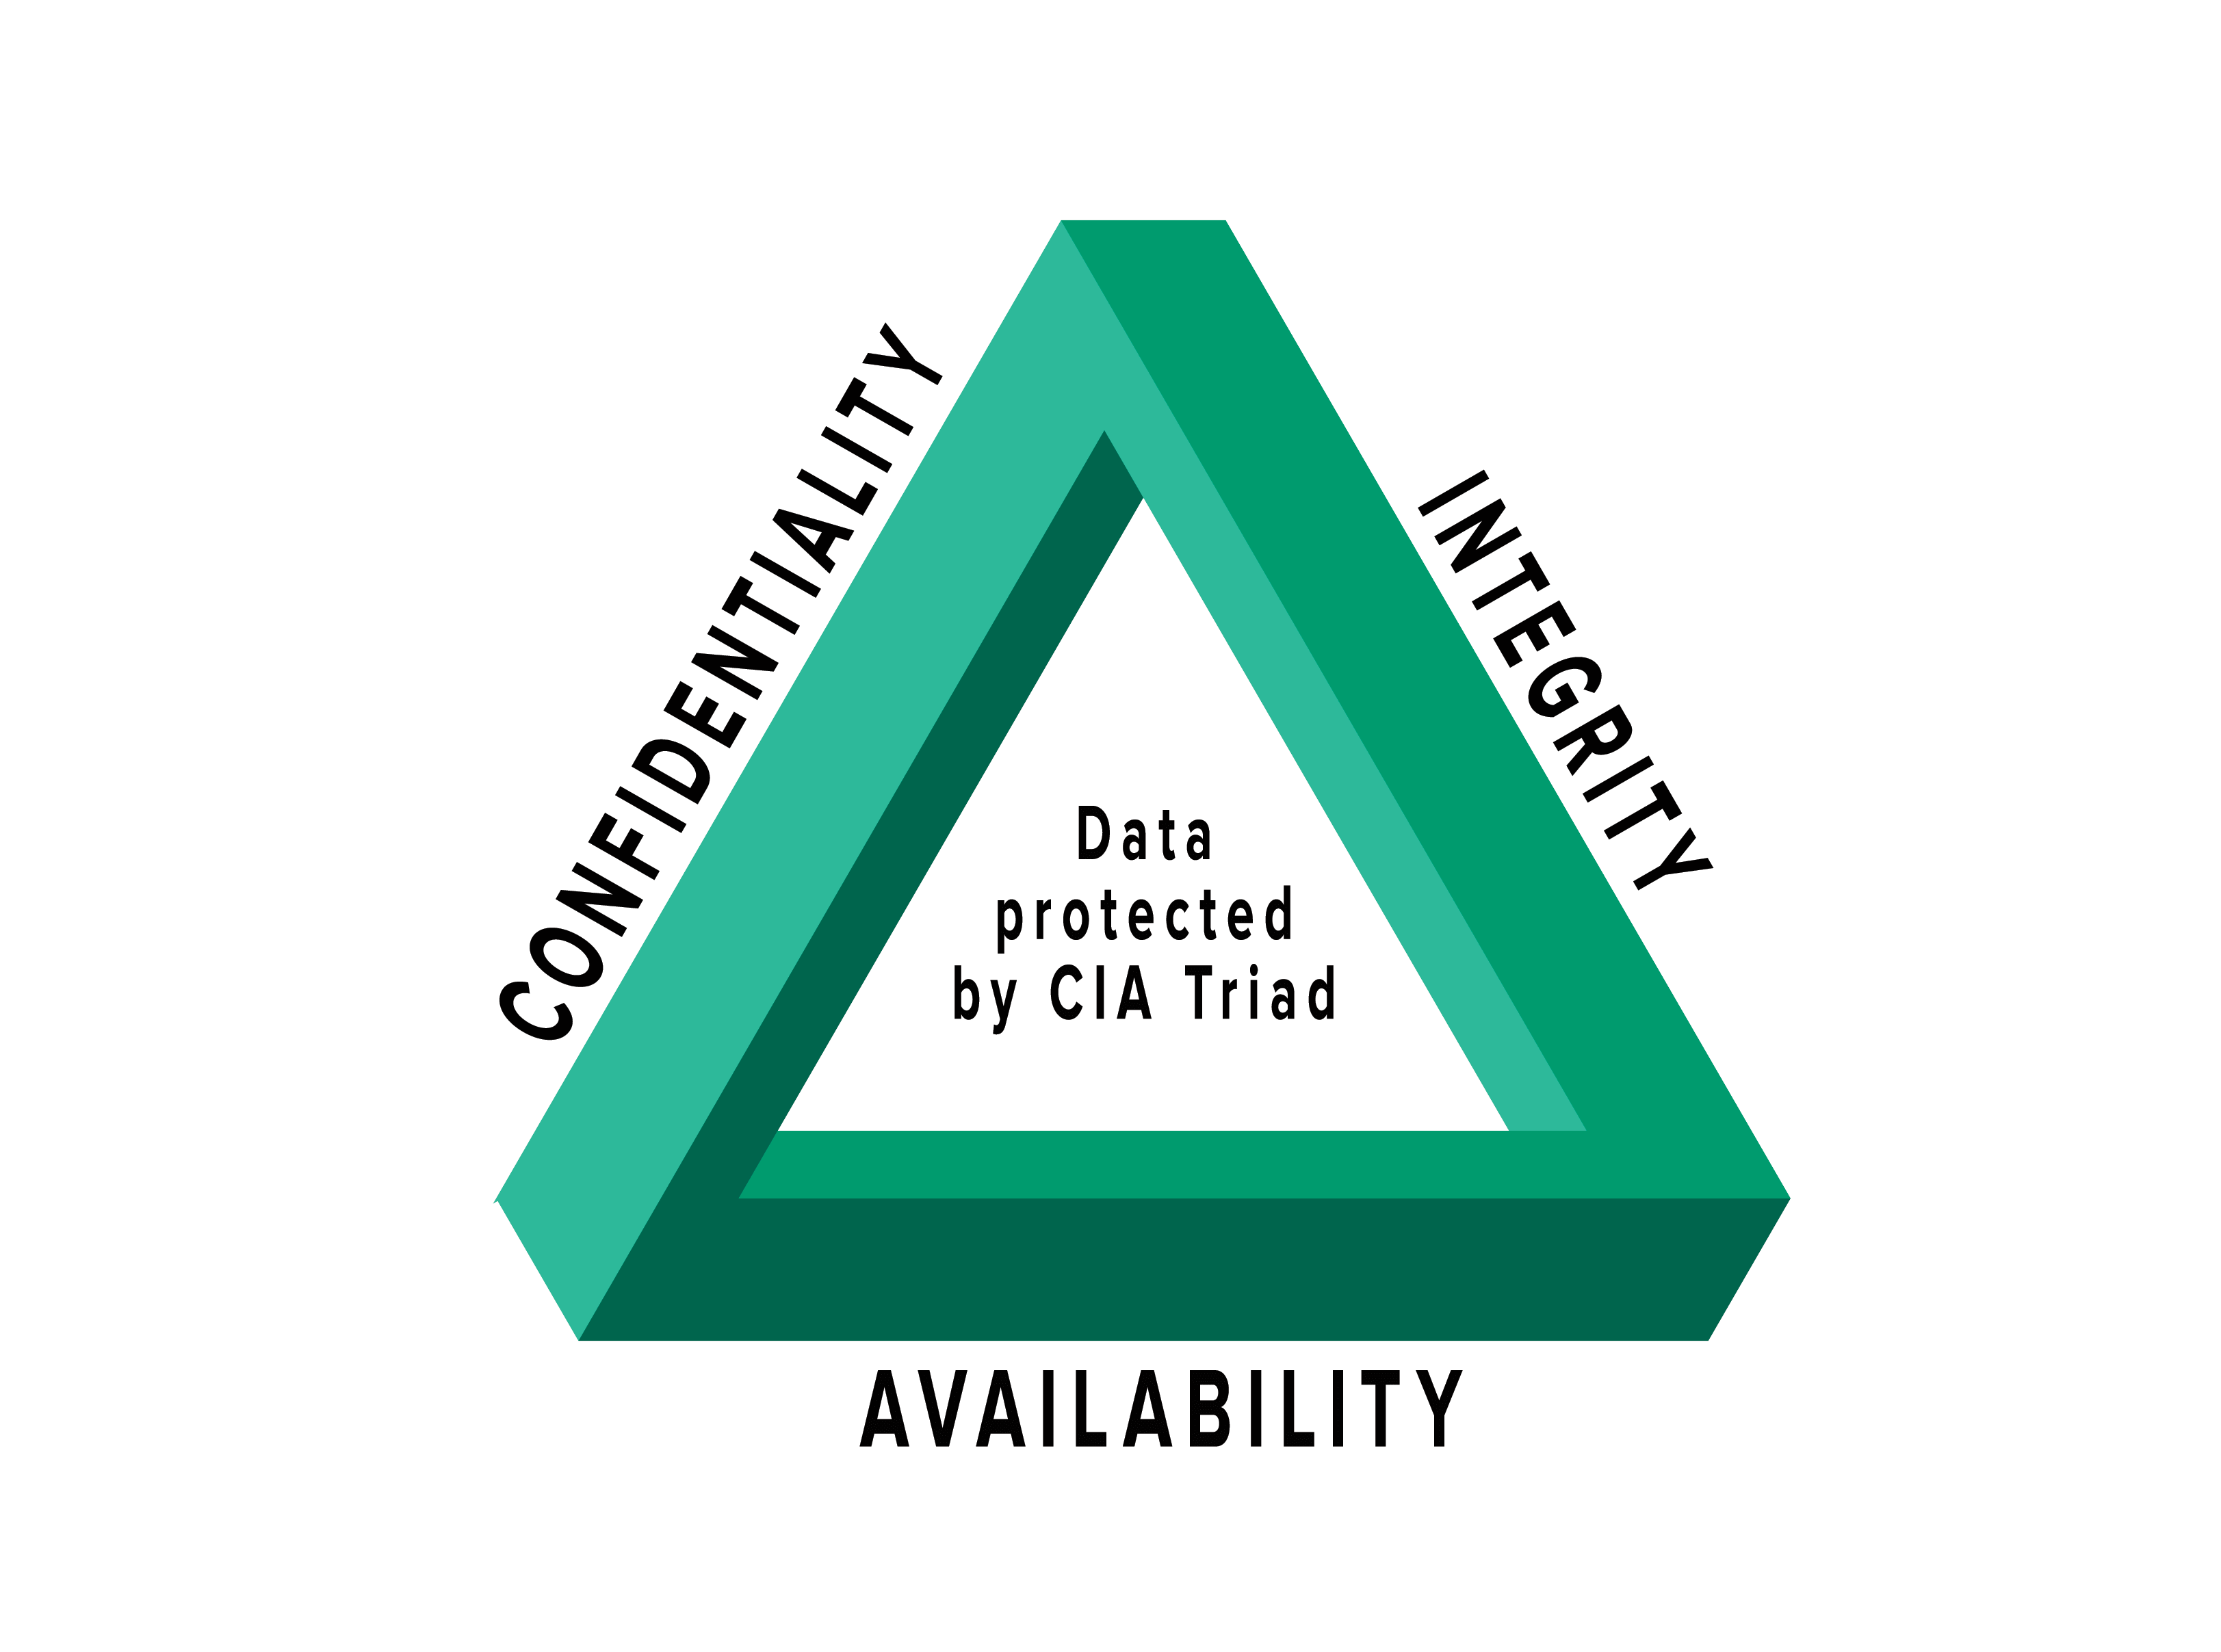
\includegraphics[width=0.8\textwidth]{images/cia_triad.png}
	\caption{CIA Triangle of Data}
	\label{fig:images-cia_triad-png}
\end{figure}
In particular,
\begin{defn}
	Confidentiality - no unauthorised disclosure
\end{defn}
\begin{defn}
	Availability - users are not denied access to resources. No unwarranted delay.
\end{defn}
\begin{defn}
	Integrity - no unauthorised change
\end{defn}
\subsection{Encryption}
Encryption is a process of securing information by covering it with an encryption and decryption key. The encryption key allows data to be stored securely, while decryption key decrypts the secured data into real data. It provides very good level security so much so that governments are worried that it might be used by criminals.
\begin{defn}
	Key escrow - Key escrow is a method of storing important cryptographic keys. Each key stored in an escrow system is tied to the original user and subsequently encrypted for security purposes.
\end{defn}
\begin{defn}
	Key disclosure - Key disclosure laws, also known as mandatory key disclosure, is legislation that requires individuals to surrender cryptographic keys to law enforcement. The purpose is to allow access to material for confiscation or digital forensics purposes and use it either as evidence in a court of law or to enforce national security interests.
\end{defn}
\subsection{the Morris Worm}
In 1988 Robert Morris exploited program bugs to write a worm. It rapidly infected $10\%$ of all machines on the Arpanet. It replicated by mistake on each machine - harm was unintentional. The worm exploited programming bugs - e.g., buffer overflow and a common 'debug' mode. Morris was issued a penalty under US 1986 Computer Fraud and Abuse Act - 3 years probation, community service and a fine of over $10,000$ USD.
\subsection{Social Engineering}
In the 1980s and 1990s Kevin Mitnick was a notorious hacker for his master of social engineering. He conned people to divulge personal information such as passwords, usually over phone. He pretended to be company's IT security group and phones human resources to get a list of new employees on the pretext of organising a security seminar. He then rings a new employee and pretends it's routine practice for security advice to be offered to new workers. During a useful discussion the hacker raised the topic and lure the employee into disclosing their password. 
\subsection{Cyxymu}
In August 2009 there was a massive DoS attack against social network sites used by Georgian Blogger 'Cyxymu'. It was one of a spate of incidents in which countries and people who were political irritations to Russia were attacked. The attack came from within Russia - there is no proof, but many pointed the finger at Russian government collusion rather than just hackers.
\subsection{Biometric Passports}
Biometric passports have been cloned to fool passport readers before:
\begin{itemize}
	\item Biometric passports are now used by many countries and the biometric information is encrypted. 
	\item In 2008, 3000 blank passports were stolen
	\item Passports have been cloned and fooled passport readers
	\item Although there is a database of passport keys, most places won't check
\end{itemize}
\subsection{Advanced Persistent Threat}
Stuxnet was a highly sophisticated worm (multiple zero-day windows sttacks, precision engineering towards particular system, rootkit, public keys stolen from several companies) and it specifically attacked Siemens' SCADA control software. It tracks were covered with a man-in-the-middle attack so that normal operation was reported.
\subsection{Hactivism}
In Jan 2012 executives of Megauploads.com were arrested and the site was taken down. Retaliation DoS attacks started within hours and Anonymous took down US government organisation websites: White House, Department of Justice, FBI. Music sites attacked too: Universal music and warner music. The attack was coordinated, decentralised and very effective.
\subsection{Physical Security}
In 2010 a computer programmer was taken hostage in Russia. He was handcuffed to a radiator and beaten to force him to hack into bank web sites. He was eventually saved by the police and the kidnappers were sentenced to 15 years in prison.
\subsection{Cyber-attacks on the increase}
The cases begin to show the diversity of computer security and the number of attacks continue to rise steadily. The proportion of UK firms reporting a cyber-attack has jumped... $55\%$ had faced an attack in $2019$, compared to $40\%$ last year.
\subsection{Terminology}
\begin{defn}
	Asset - anything we value and want to protect
\end{defn}
\begin{defn}
	Vulnerability - a flaw or weakness in a system's design, implementation or operation and management that could be exploited to violate the system's security policy.
\end{defn}
\begin{defn}
	Threat - a potential for violation of security, which exists when there is a circumstance, capability, action or event that could breach security and cause harm
\end{defn}
\begin{defn}
	Attack - an assault on system security that derives from an intelligent threat i.e., an intelligent act that is a deliberate attempt to evade security services and violate the security police of a system.
\end{defn}
\begin{defn}
	Risk - an expectation of loss expressed as the probability that a particular threat will exploit a particular vulnerability with a particular harmful result. 
\end{defn}
\begin{defn}
	Countermeasure - an action, device, procedure or technique that reduces a threat, vulnerability or attack by eliminating or preventing it, by minimising the harm it can cause, or by discovering and reporting it as that corrective action can be taken.
\end{defn}
\begin{defn}
	Risk assessment
	\begin{align*}
\text{Exposure} = \text{Assets} \times  \text{Threats} \times \text{Vulnerabilities}
	\end{align*}
\end{defn}
\section{Organisations}
\subsection{Legal Entity}
\begin{defn}
	Legal entity - is an individual, company or organisation that has legal rights and obligations. It can be entered into contracts, be taken to court etc.
\end{defn}
\begin{defn}
	Unlimited liability - you can lose everything i.e., there is no limit on how much you can be sued for
\end{defn}
Some examples of legal entities include:
\begin{itemize}
	\item Sole trader
	\item Partnership
	\item Corporation
	\item Cooperatives
\end{itemize}
\subsection{Creating a corporation}
A company can be created through
\subsubsection{Royal Charter}
Organisations used to be created in a simple - whoever was governing issued a document creating that organisation. The University of Warwick was created by a Royal Charter.
\subsubsection{Act of Parliament}
Organisations can be created through an Act of Parliament e.g., governing institutions, councils, some statutory companies
\subsubsection{Companies Act}
Most organisations are limited companies that are created through the Companies Act
\subsection{Limited Companies}
\subsubsection{Public Limited Company (PLC)}
PLCs can sell shares to general public - shares and bonds. This means that its stocks are traded on stock exchange. Must adhere to regulations and reporting standards and can be vulnerable to takeovers.
\subsubsection{Private Limited Company (LTD)}
Shares aren't traded but can be sold to private investors or venture capitalists. Stocks traded between investors and there are fewer regulations e.g., $<500$ shareholders and $<10$ million USD.
\subsection{Memorandum of Association}
Up until 30 September 2009 two documents were created one of which was the memorandum of association. Included stuff are:
\begin{itemize}
	\item Name, registered office and country - all included in detail
	\item Company activities - explained very broadly e.g., trading
	\item Liability clause - how the liability is carried out, e.g., limited by shares or guarantee
	\item Share capital - money initially invested
	\item Declaration of association - statement from initial investors
\end{itemize}
In the articles of association prior to $2009$, the included stuff are:
\begin{itemize}
	\item Dividends
	\item Board Meetings
	\item Membership of board of directors
	\item Directors' terms of office
	\item Sales of shares
	\item Directors' powers
\end{itemize}
After 1st October, the framework changed slightly. The Companies (Model Articles) Regulations 2008 replaced "Table A".
\begin{defn}
	Table A - the first document that was presented originally. It contained detail about how the business is conducted, shares are traded, directors are elected etc.
\end{defn}
The memorandum was subsumed into the Articles and is no longer part of the company's constitution. Now companies require the articles of association.
\subsection{Organisational Models}
\subsubsection{Bureaucratic model}
\begin{enumerate}
	\item All tasks are split into specialised jobs in which jobholders become exxpert
	\item The performance of each task is governed by precise rules
	\item In order to ensure that personalities and personal relationships do not interfere with performance, employees are required to relate both to other employees and to clients in an impersonal and formal manner
	\item Recruitment is based on qualifications and employees are protected against arbitrary dismissal.
\end{enumerate}
\subsubsection{The Organic Model}
An organisation will be effective to the extent that its structure is such as to ensure a maximum probability that in all interactions and in relationships within the organisation, each member, in the light of his background, values, desires, and expectations, will view the experience as supportive and one which builds a sense of personal worth and importance.
\subsubsection{Matrix Management}
In the past 30 years or so the idea of matrix management has become more fashionable as a way of addressing cases where employees may have more than a single manager. It is a method trying to resolve the conflict between them. In software company, for example, database specialists may belong to a database group and report to its manager, while at the same time reporting to the project manager of the project they are working on. 

\subsection{2008 Financial Crisis}
The 2008 financial crisis highlights the risk of companies and organisations. It was caused by an increase in the risky practice of lending for sub prime mortgages.
\begin{defn}
	Subprime - refers to borrowers or loans, usually offered at rates well above the prime interest rate, that have poor credit ratings. Subprime lending is higher risk, given the lower credit rating of borrowers, and has in the past contributed to financial crises.
\end{defn}
In September 2008, Lehman Brothers, a US investment bank went bust. Bailouts were necessary to prevent further collapse.
\subsection{Structuring Principles}
The structuring principles is a way to dissect how big companies are put together. 
\begin{itemize}
	\item By Function - medium sized organisations are often structured by function. In a typical company, departmental functions include production, finance, quality, marketing, research and development and human resources. A legal team may also exist if it is big enough
	\item By Location - For large companies where local knowledge and local regulations play a big part, such as multinationals and banks, structuring by location may be used
	\item By Product - structuring by product works where there is clear product differentiation.
	\item By market sector - Structuring by market sector works for example for service products, where there is clear sector differentiation (e.g. window cleaning for private individuals and window cleaning for large organisations).
	\item By technology - An example of a company structured by technology is IBM, which is used to produced PCs, mainframes and operating systems that could be separated. However it's not so easy to structure by technology now, although it make sense occasionally.
\end{itemize}
There are also structural considerations which include:
\begin{itemize}
	\item Operational structure - by project e.g., if objectives need to be achieved by a specific deadline or by production e.g., specific activities managed by a single team
		\item Depth of Structure - Companies choose a chain of command which is effective. The bigger the company, the more likely it is to have more layers of management.
		\item Centralisation - (making the top control more in the hierarchy) is appropriate for company wide policies, for example corporate branding for a consistent look and feel.
\end{itemize}
\subsection{Job design}
\begin{defn}
	Job enrichment - redesigning jobs so that the amount of responsibility, discretion and control required of the employee is increased
\end{defn}
\begin{defn}
	Job rotation - rotating staff through a series of jobs to prevent employees from becoming bored with a very narrow and specialised task
\end{defn}
\begin{defn}
	Job enlargement - redesign of a job so that it includes more tasks which require essentially the same level of skill and responsibility
\end{defn}
\section{Companies}
\subsection{Starting a company}
A starting company requires:
\begin{itemize}
	\item Capital - i.e., money
	\item Cash flow - i.e., money coming in and out
	\item Sources of finance - i.e., equity capital, loans etc.
	\item Gearing - ratio of loan capital to equity
\end{itemize}
\begin{defn}
	Grants - sum of money given to a company by the government
\end{defn}
\begin{defn}
	Loans - sum of money lent to a company
\end{defn}
\begin{defn}
	Equity Capital - money paid to the company in exchange for a share in the ownership of the company. Usually venture capitalists or business angels use this method for companies with good prospects
\end{defn}
\begin{defn}
	Gearing / leverage - the relationship between loan capital and equity capital. High levels of gearing is generally undesirable.
\end{defn}
\subsection{Balance Sheet}
A balance sheet has:
\begin{itemize}
	\item Assets - i.e., what a company owns, current vs. fixed, depreciation and debtors
	\item Liabilities - i.e., what a company owns and creditors
	\item Net Worth - i.e., assets minus liabilities
\end{itemize}
\subsection{Profit and Loss Account}
A profit and loss account has:
\begin{itemize}
	\item Approximation: during a single year i.e., $\text{Change in net worth}=\text{income}-\text{expenditure}$
	\item Need to consider cash flow i.e., how the cash moves about
	\item Also need to consider depreciation and monies owing.
\end{itemize}
\subsection{Cash Flow statement}
Movement of cash (excludes non-cash transactions, such as depreciation) including but not limited to:
\begin{itemize}
	\item Interest payments
	\item Tax
	\item Dividends to shareholders
	\item Capital expenditure
	\item Disposals
\end{itemize}
\subsection{Relationship between them}
\begin{figure}[H]
	\centering
	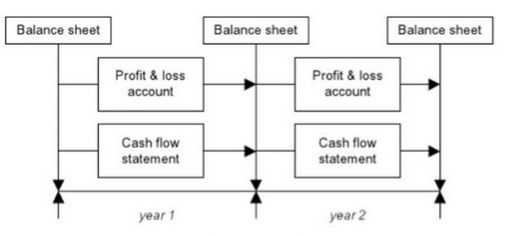
\includegraphics[width=0.6\textwidth]{images/relation.png}
	\caption{Relationship between Cash Flow, Profit and Loss and Balance Sheet}
	\label{fig:images-relation-png}
\end{figure}
The relationship is that Balance sheet happens at the end of each year. Profit and loss account along with Cash Flow statement happens throughout year, for which is then used to generate the balance sheet next year.
\subsection{Double Entry Bookkeeping}
Conceptually, pages in a book. Every single entry appears "twice". The idea is that through ledgers you are able to make sure that when you add specific things e.g., orders, the add up correctly since you take record twice.
\begin{figure}[H]
	\centering
	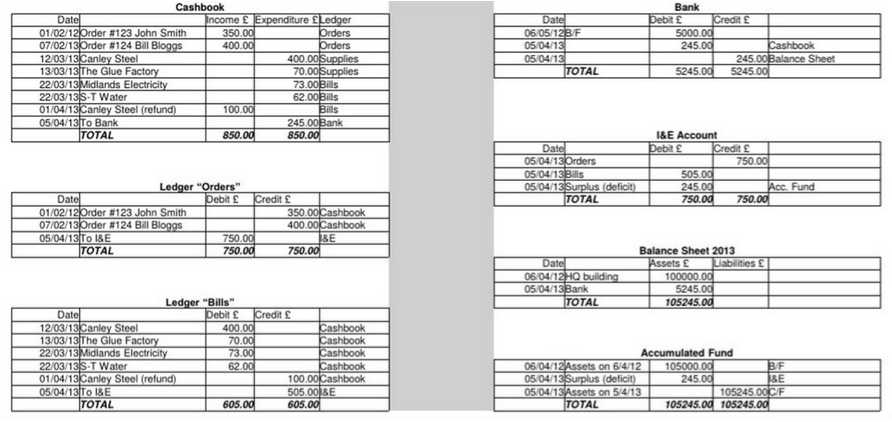
\includegraphics[width=0.8\textwidth]{images/doubleentry.png}
	\caption{Double Entry Bookkeeping}
	\label{fig:images-doubleentry-png}
\end{figure}
\subsection{Accounts and Budgetes}
\begin{defn}
	Accounts - these tell you what happened
\end{defn}
\begin{defn}
	Budgets - tell you what you expect to happen
\end{defn}
\begin{defn}
	Direct costs - things that include directly in the production of a product e.g., raw materials, shipment
\end{defn}
\begin{defn}
	Indirect costs - things that are not directly in the production of a product e.g., utility bills, wages, rent
\end{defn}
\subsection{Labour}
Labour includes:
\begin{itemize}
	\item Salaries i.e., monthly, weekly or hourly, Income Tax (PAYE), Pension contributions and national insurance contributions.
	\item Days off sick i.e., statutory sick pay
\end{itemize}
		\subsection{Overheads}
		\begin{defn}
			Overheads - expenses you can't avoid	
		\end{defn}
		These include
		\begin{itemize}
			\item Rental
			\item Vehicles
			\item Bills
			\item Telecomms
			\item Postage
			\item Insurance
		\end{itemize}
		\subsection{Investment}
		The Discounted cash flow analysis includes the return on investment and the interest rate $r\%$ over $t$ years, given with a discount factor
		\begin{align*}
			\frac{1}{(1+r)^{t}}
		\end{align*}
It also includes the rate of return. However, since this is forecasting there are some inherent problems:
\begin{itemize}
	\item Market Conditions
	\item Competitors
	\item Credit availability
	\item Interest rates
\end{itemize}
which can all change.
\subsection{Statutory requirements}
Annual returns and accounts MUST be filed to the Companies House and sent to HMRC. Accounts must audited if the company is large enough and must also contain balance sheet, profit and loss account, notes on the accounts and directors' report if it is large enough.
\begin{defn}
	Insolvency - trading with a company that did not break even over a period of time or is not in a position insolvently and it is bankrupt. 
\end{defn}
\section{Contracts and Human Resources}
\subsection{Contracts}
\begin{defn}
	Contract -  a legal agreement between two or more parties which must:
	\begin{itemize}
		\item Be competent
		\item Intend to make the contract
		\item Receive/provide a consideration
	\end{itemize}
\end{defn}
and contracts can be broken down into two:
\begin{enumerate}
	\item The main agreement - this includes the signatures
	\item The schedules - this details the tasks and actions associated with the contract
\end{enumerate}
\subsection{The Schedule}
The schedule must include:
\begin{enumerate}
	\item What is to be supplied
	\item Price, deadlines, payment terms
	\item Legal rights - who owns the intellectual property
	\item Confidentiality
	\item Delays, changes, penalty causes - e.g., if the project overruns
	\item Client obligations - Logistics and hardware i.e., where will it be written
	\item Milestones - Key targets to ensure that the software development life cycle is on track
	\item Acceptance procedures - how is it defined if the development is complete
	\item Warranty, maintenance - responsibility for fixing errors if they arise
	\item Indemnity - what happens if use of the software results in damage
	\item Termination - grounds at which the contract can be ended
	\item Arbitration - the mechanism for resolving disputes between the parties
	\item Applicable law - If in court, which law applies e.g., UK, US etc.
\end{enumerate}

\subsection{Consultancy contracts}
The following terms are to especially watch out for:
\begin{defn}
	Liability - who is responsible
\end{defn}
\begin{defn}
	Confidentiality - who can view, gain information
\end{defn}
\begin{defn}
	Terms of reference - purpose and structures of the contract and the deal
\end{defn}
\begin{defn}
	Control over deliverables - e.g., who initiates, plans, closes etc.
\end{defn}
\subsection{Human resources}
Human resources consists of:
\begin{itemize}
	\item Recruitment and selection - processes for recruiting new employees into the organisation, job descriptions to define their duties and employment contracts to attribute rights and responsibilities to the organisation and employee.
	\item Redundancies, dismissal and grievances - Similarly,  they should have define for the above definition
	\item Staff support $\&$ development - To keep employee retention rates high, organisations need to help staff enhance their skills, which in turn benefits both employee and employer.
\end{itemize}
\begin{defn}
	Appraisals - to help ensure staff are progressing in their job and that their skills are up-to-date, organisations should undertake regular monitoring meetings with employees
\end{defn}
\begin{defn}
	Remuneration policy - how salary is calculated and how employees can be incentivised
\end{defn}
\begin{defn}
	Employment acts - Human rights act 1998, Equality act 2006, Equality act 2010
\end{defn}
\subsection{Discrimination}
Organisations are not allowed to discriminate. They are not allowed to discriminate against anyone because of the protected characteristics:
\begin{itemize}
	\item Age
	\item Gender reassignment
	\item Being married or in a civil partnership
	\item Being pregnant or on maternity leave
	\item Disability
	\item Race including colour, nationality, ethnic or national origin
	\item Religion or belief
	\item Sex
	\item Sexual orientation
\end{itemize}
The same applies with software and web access, by Web Content Accessibility Guidelines (WCAG)
\subsection{Athena Swan Charter}
The Athena SWAN charter is a framework used across the global to support and transform gender equality within higher education and research. It was established in 2005 to encourage and recognise commitment to advancing careers of women in STEMM employment.
\subsection{Me too movement}
A me too movement against sexual harassment and assault based on breaking silence was made. It's purpose was to empower women by visibly demonstrating the extent of sexual harassment in the workplace.
\end{document}
